\documentclass[compress]{beamer}
\usepackage{ifthen,verbatim}

\title{MuonHIP Alignment Results}
\author{Jim Pivarski, Alexei Safonov}
\institute{Texas A\&M University}
\date{28 May, 2008}

\newcommand{\isnote}{}
\xdefinecolor{lightyellow}{rgb}{1.,1.,0.25}
\xdefinecolor{darkblue}{rgb}{0.1,0.1,0.7}

%% Uncomment this to get annotations
%% \def\notes{\addtocounter{page}{-1}
%%            \renewcommand{\isnote}{*}
%% 	   \beamertemplateshadingbackground{lightyellow}{white}
%%            \begin{frame}
%%            \frametitle{Notes for the previous page (page \insertpagenumber)}
%%            \itemize}
%% \def\endnotes{\enditemize
%% 	      \end{frame}
%%               \beamertemplateshadingbackground{white}{white}
%%               \renewcommand{\isnote}{}}

%% Uncomment this to not get annotations
\def\notes{\comment}
\def\endnotes{\endcomment}

\setbeamertemplate{navigation symbols}{}
\setbeamertemplate{headline}{\mbox{ } \hfill
\begin{minipage}{5.5 cm}
\vspace{-0.75 cm} \small
\end{minipage} \hfill
\begin{minipage}{4.5 cm}
\vspace{-0.75 cm} \small
\begin{flushright}
\ifthenelse{\equal{\insertpagenumber}{1}}{}{Jim Pivarski \hspace{0.2 cm} \insertpagenumber\isnote/\pageref{numpages}}
\end{flushright}
\end{minipage}\mbox{\hspace{0.2 cm}}\includegraphics[height=1 cm]{../cmslogo} \hspace{0.1 cm} \includegraphics[height=1 cm]{../tamulogo} \hspace{0.01 cm} \vspace{-1.05 cm}}

\begin{document}
\frame{\titlepage}

%% \begin{notes}
%% \item This is the annotated version of my talk.
%% \item If you want the version that I am presenting, download the one
%% labeled ``slides'' on Indico (or just ignore these yellow pages).
%% \item The annotated version is provided for extra detail and a written
%% record of comments that I intend to make orally.
%% \item Yellow notes refer to the content on the {\it previous} page.
%% \item All other slides are identical for the two versions.
%% \end{notes}

\begin{frame}
\frametitle{Summary}

\begin{itemize}\setlength{\itemsep}{0.3 cm}
\item Goal for S156: ``few hundred microns'' in first muon stations (ultimate goal is 200~$\mu$m with 100~pb$^{-1}$)
\item First time we saw low-$p$ muon \mbox{samples (MuonPT5, MuonPT11)\hspace{-1 cm}}
\item Learned that alignment quality optimized by \mbox{low $p_T$ cut (10~GeV)\hspace{-1 cm}}
\item Achieved: 500--800~$\mu$m in first muon stations in S156 (10~pb$^{-1}$), scale by $\sqrt{10}$ $\to$ 250~$\mu$m at 100~pb$^{-1}$
\item Strong dependence on tracker alignment
\item Pointing resolution depends on $L_{\mbox{\scriptsize muon}} / L_{\mbox{\scriptsize tracker}}$ (negligible),

curvature resolution depends on $(L_{\mbox{\scriptsize muon}} / L_{\mbox{\scriptsize tracker}})^2$ (important)
\item Tracker momentum resolution should scale with statistics, since it is optimized by alignments to $Z\to\mu\mu$ mass constraints
\end{itemize}
%% \hspace{-0.83 cm} \textcolor{darkblue}{\Large Outline2}
\end{frame}

\begin{frame}
\frametitle{Barrel aligned positions ($r\phi$)}
\small

Grey: misaligned (1.5~mm), yellow: aligned (680~$\mu$m), \\ dashed: if tracker were ideal (300~$\mu$m)

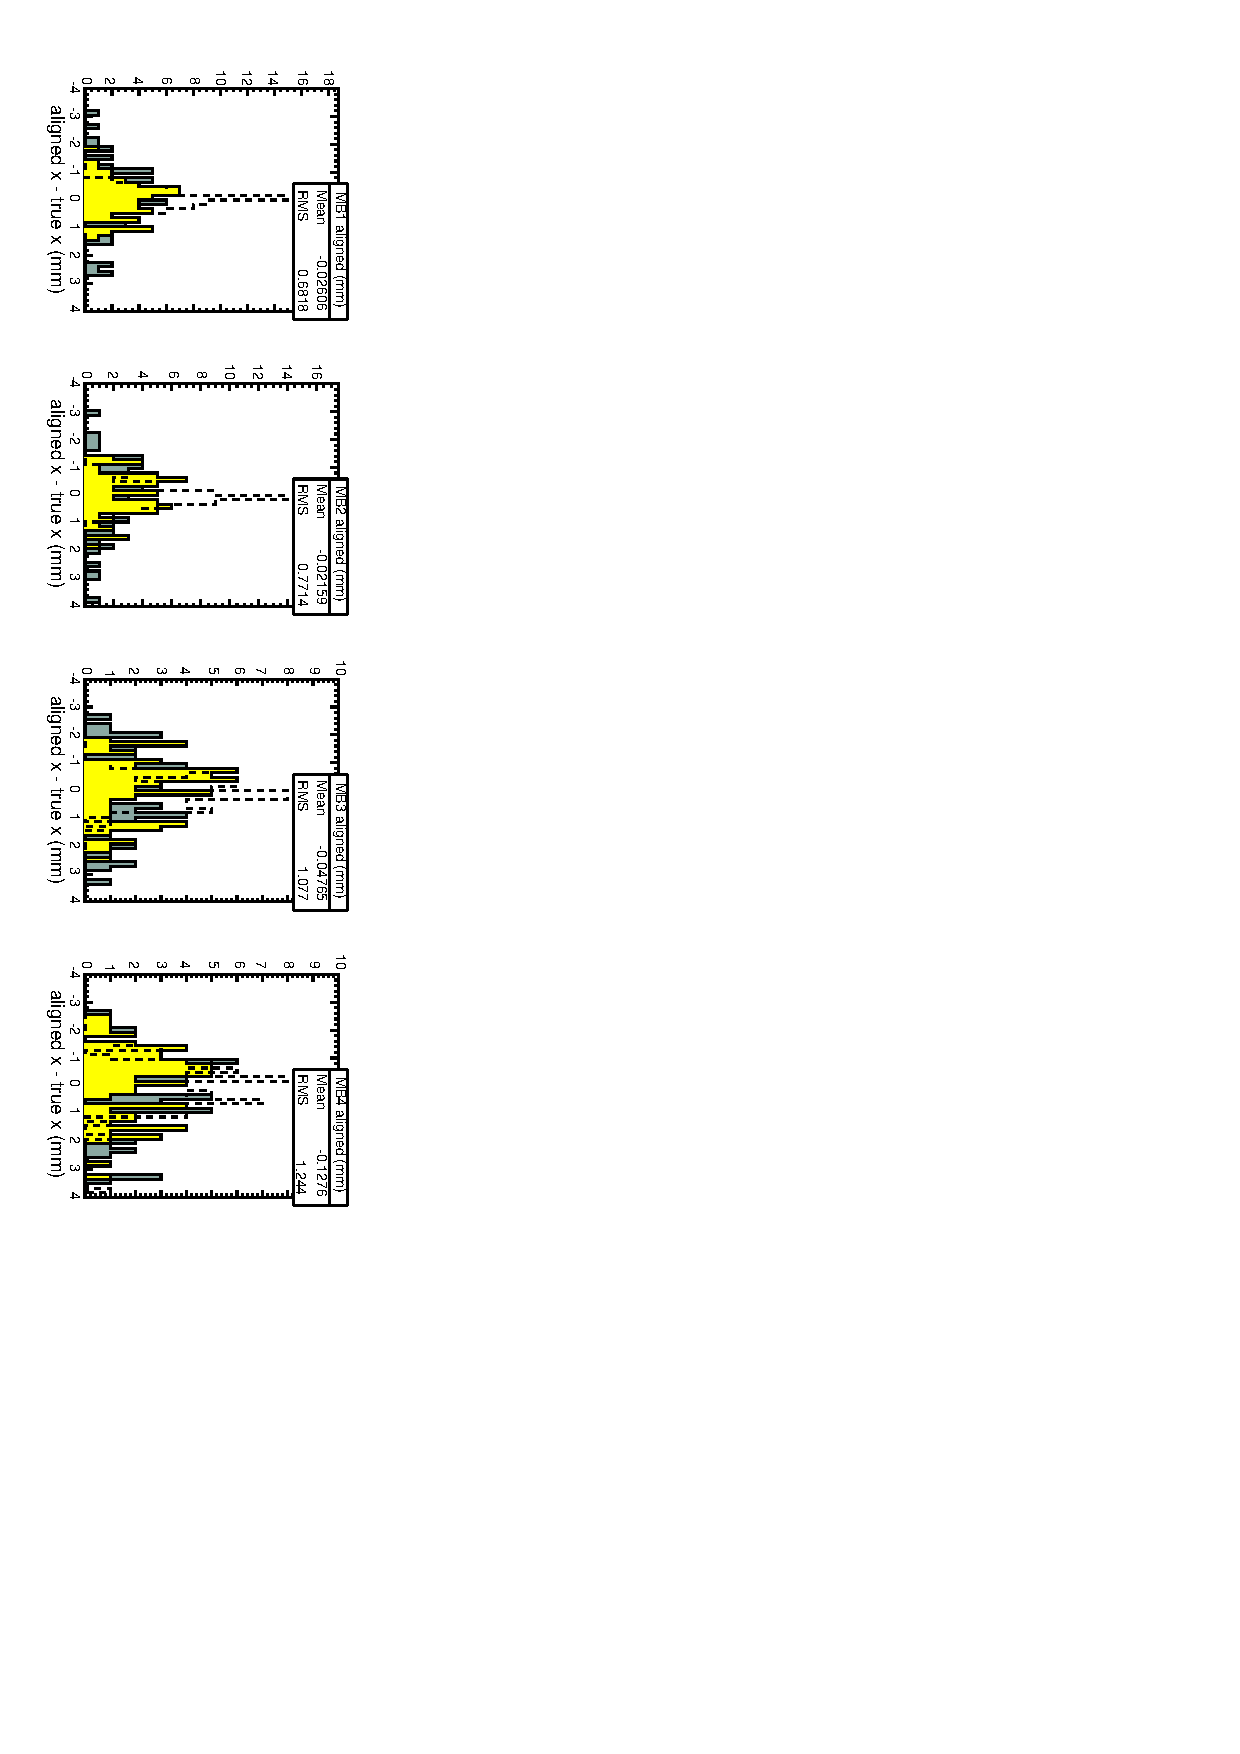
\includegraphics[height=\linewidth, angle=90]{muonhip_barrelx.pdf}

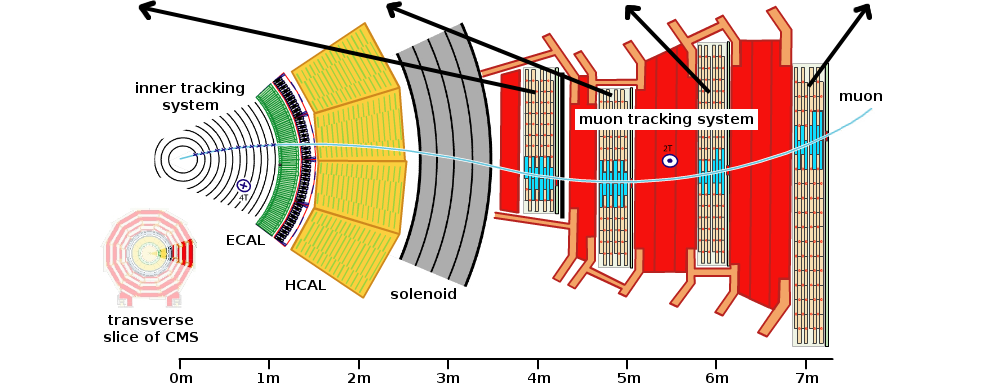
\includegraphics[width=\linewidth]{cms_slice.png}
\end{frame}

\begin{frame}
\frametitle{Endcap aligned positions ($r\phi$)}
\small
Best results in inner ring (bottom row), where $L_{\mbox{\scriptsize muon}}$ $\sim$ $L_{\mbox{\scriptsize tracker}}$

\vfill
\begin{columns}
\column{0.35\linewidth}
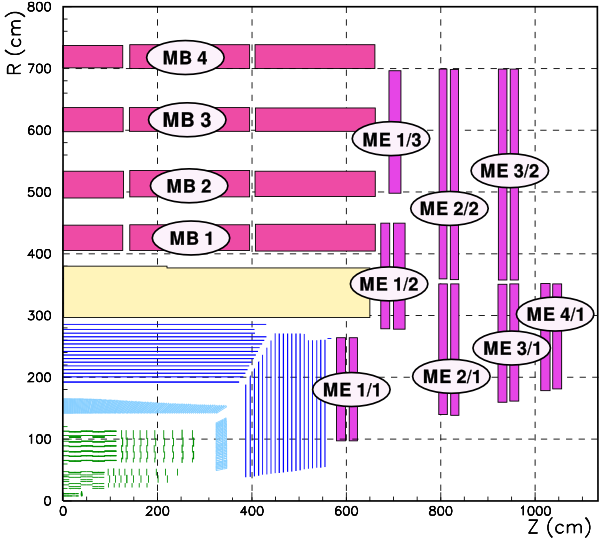
\includegraphics[width=\linewidth]{muon_system.png}
\column{0.8\linewidth}
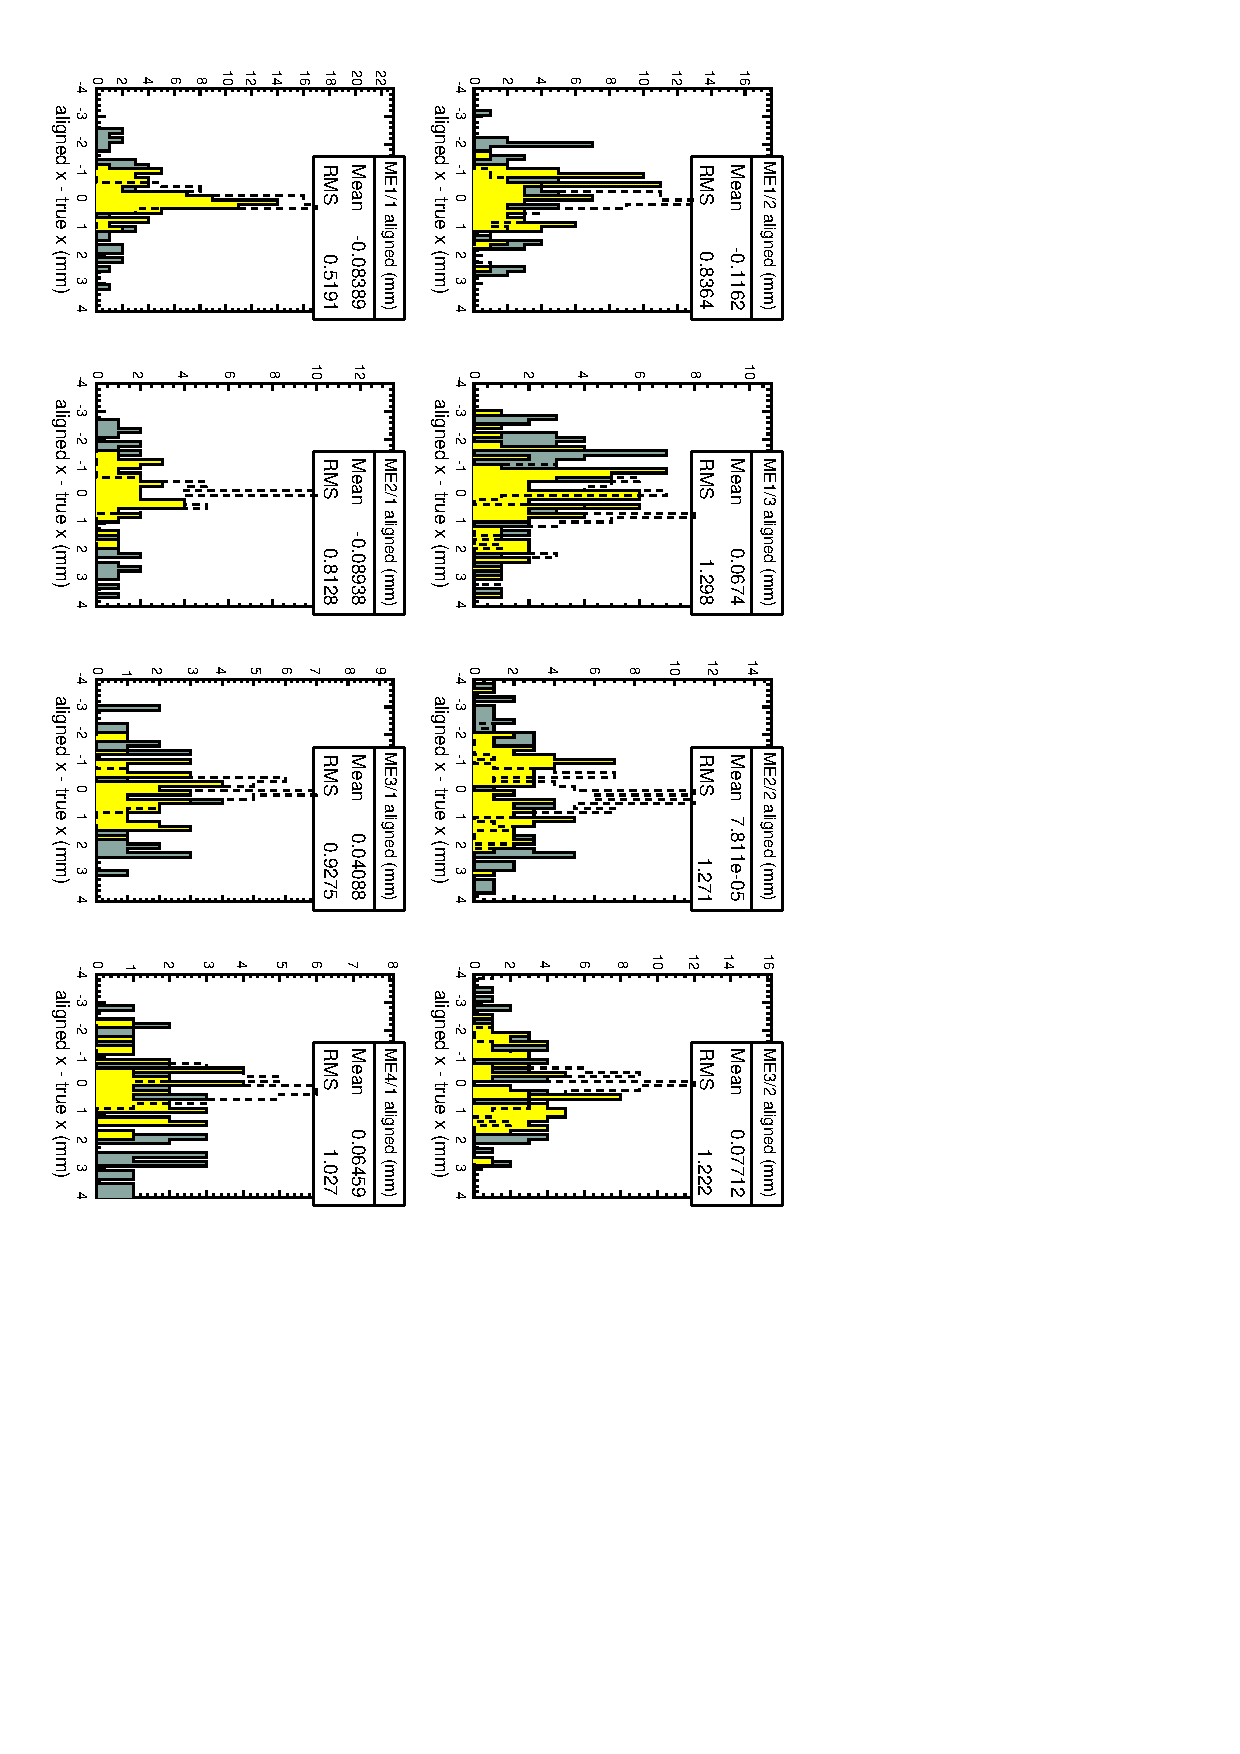
\includegraphics[height=\linewidth, angle=90]{muonhip_endcapx.pdf}
\end{columns}

\end{frame}


%% \section*{First section}
%% \begin{frame}
%% \begin{center}
%% \Huge \textcolor{blue}{First section}
%% \end{center}
%% \end{frame}

\begin{frame}
\frametitle{Conclusions}

\begin{itemize}\setlength{\itemsep}{0.5 cm}
\item Successful exercise from several points of view
\begin{itemize}\setlength{\itemsep}{0.2 cm}
\item Resolution equal to or better than initial misalignment in all stations and all parameters
\item Would scale appropriately to 100~pb$^{-1}$ goals
\item Clarified exactly how muon alignment depends on tracker
\item Learned how to use low-$p$ muons (previously, an open question)
\item Alignment machinery has matured quite a bit, added cuts against rare bad tracks discovered in the exercise
\item Included studies of how to use data to assess alignment quality (not shown here)
\end{itemize}

\item Aligned constants used in S156 re-reconstruction

\item Working on twiki page!
\end{itemize}

\label{numpages}
\end{frame}

\end{document}
